\documentclass[8pt]{beamer}
\usepackage{tikz}
\usepackage{amssymb}
\usepackage{graphicx}
\usepackage{wasysym}
\usepackage{spverbatim}
\usepackage{natbib}
\usepackage{dsfont}
\usepackage{lmodern}
\setcitestyle{square}
\usepackage{float}
\usepackage{amsmath}
\usepackage{amscd}
\usepackage{hyperref}
\usepackage{enumerate}
\usepackage{amsfonts}
\usepackage{amssymb}
\usepackage[utf8]{inputenc}
\usepackage{amsthm}	
\usepackage{caption}
\usepackage{subcaption}
\usepackage{booktabs}
\usepackage{booktabs}
\usepackage{colortbl}
\usepackage{nameref}
\usepackage{multirow}
\usepackage{animate}
\usetikzlibrary{arrows,decorations.pathmorphing,backgrounds,positioning,fit,matrix, calc, quotes, angles, decorations.pathreplacing}
\usepackage{tikz-cd}
\usepackage{wrapfig}
\tikzset{node distance=2cm, auto}
%PARA el gif
\usepackage{animate}
%Para los comentarios
\usepackage{comment}


  \usetheme{Madrid}       % or try default, Darmstadt, Warsaw, ...
  \usecolortheme{default} % or try albatross, beaver, crane, ...
  \usefonttheme{serif}    % or try default, structurebold, ...
  \setbeamertemplate{navigation symbols}{}
  \setbeamertemplate{caption}[numbered]




\newcommand{\vspan}[1]{\text{span}\left\lbrace #1\right\rbrace}
\newcommand{\dual}[2]{\left\langle #1 , #2\right\rangle}
\def\quotient#1#2{%
    \raise1ex\hbox{$#1$}\big/\hbox{$#2$}%
}

\newcommand{\norm}[1]{\left|\left| #1\right|\right |}

\newcommand{\ultra}[1]{\left( #1\right)_\mathcal{U}}

\newenvironment{variableblock}[3]{%
  \setbeamercolor{block body}{#2}
  \setbeamercolor{block title}{#3}
  \begin{block}{#1}}{\end{block}}
  
  
\graphicspath{{./Figuras/}} 

\usepackage{listings}
\usepackage{color}
\definecolor{dkgreen}{rgb}{0,0.6,0}
\definecolor{gray}{rgb}{0.5,0.5,0.5}
\definecolor{mauve}{rgb}{0.58,0,0.82}

\lstset{ %
  language=R,                     % the language of the code
  basicstyle=\footnotesize,       % the size of the fonts that are used for the code
  numbers=left,                   % where to put the line-numbers
  numberstyle=\tiny\color{gray},  % the style that is used for the line-numbers
  stepnumber=1,                   % the step between two line-numbers. If it's 1, each line
                                  % will be numbered
  numbersep=5pt,                  % how far the line-numbers are from the code
  backgroundcolor=\color{white},  % choose the background color. You must add \usepackage{color}
  showspaces=false,               % show spaces adding particular underscores
  showstringspaces=false,         % underline spaces within strings
  showtabs=false,                 % show tabs within strings adding particular underscores
  frame=single,                   % adds a frame around the code
  rulecolor=\color{black},        % if not set, the frame-color may be changed on line-breaks within not-black text (e.g. commens (green here))
  tabsize=2,                      % sets default tabsize to 2 spaces
  captionpos=b,                   % sets the caption-position to bottom
  breaklines=true,                % sets automatic line breaking
  breakatwhitespace=false,        % sets if automatic breaks should only happen at whitespace
  title=\lstname,                 % show the filename of files included with \lstinputlisting;
                                  % also try caption instead of title
  keywordstyle=\color{blue},      % keyword style
  commentstyle=\color{dkgreen},   % comment style
  stringstyle=\color{mauve},      % string literal style
  escapeinside={\%*}{*)},         % if you want to add a comment within your code
  morekeywords={*,...}            % if you want to add more keywords to the set
} 

%%%%%%%%%%%%%%%%%%%%%%%%%%%%%%%%%%%%%%%%%%%%%%%%%%%%%%%%%%%%%%%%%%%%%%%%%%%%%%%%%%%%%%%%%%%%%%%%%%%%%%%%%%%%%%%%%%%%%%%%%%%%%%%%%%%%%%%%%%%%%%%%%%%%%%%%

\AtBeginSection[]{
  \begin{frame}
  \vfill
  \centering
  \begin{beamercolorbox}[sep=8pt,center,shadow=true,rounded=true]{title}
    \usebeamerfont{title}\insertsectionhead\par%
  \end{beamercolorbox}
  \vfill
  \end{frame}
}

\title{Métodos estadísticos y de inferencia causal}


\author{Isaac Meza López\inst{1}}
% - Give the names in the same order as the appear in the paper.
% - Use the \inst{?} command only if the authors have different
%   affiliation.

\institute[ITAM] % (optional, but mostly needed)
{
  \inst{1}%
  ITAM
  
}
% - Use the \inst command only if there are several affiliations.
% - Keep it simple, no one is interested in your street address.

\date{Junio 2019}
% - Either use conference name or its abbreviation.
% - Not really informative to the audience, more for people (including
%   yourself) who are reading the slides online

\subject{Econometría}
% This is only inserted into the PDF information catalog. Can be left
% out. 

% If you have a file called "university-logo-filename.xxx", where xxx
% is a graphic format that can be processed by latex or pdflatex,
% resp., then you can add a logo as follows:



% Let's get started


\begin{document}

\begin{frame}
  \titlepage
\end{frame}

%These three lines create an automatically generated table of contents.
\begin{frame}[allowframebreaks]{Contenidos}
  \tableofcontents
\end{frame}

\nocite{*}
\begin{frame}[allowframebreaks]{Lectura sugerida}
\bibliographystyle{amsalpha}
\bibliography{References}
\end{frame}

\begin{frame}{Dropbox}
    Los materiales y ésta presentación la pueden encontrar \color{blue}\href{https://github.com/isaacmeza/metodos_estadisticos}{aquí}.
\end{frame}


\section{Diseño de experimentos}
%Todos los diseños Pilot3 - Notificaciones
\subsection{Simulación de poder}
\begin{frame}[allowframebreaks]{Simulación de Poder}
    Poder estadístico $(1-\beta$) es la verosimilitud/probablidad de detectar cierto efecto cuando hay un efecto que detectar.\\
    
    \[H_0\;:\;\theta = 0\]
    \[H_1\;:\;\theta \neq 0\]
    
    \[1-\beta = Pr(\text{rechazar } H_0\;|\;H_1 \text{ es verdadera}) \]
    
   
\begin{table}[H]
  \centering
    \begin{tabular}{l|cc}
    \toprule
    \multicolumn{1}{r}{Concluir} & \multicolumn{2}{c}{Realidad} \\
    \midrule
    \midrule
     & $H_0$ TRUE & $H_0$ FALSE \\
     \midrule
    \multicolumn{1}{c|}{$H_0$ TRUE} & $(1-\alpha)$ & Type I : $\beta$ \\
    $H_0$ FALSE & Type II: $\alpha$ & $(1-\beta)$ \\
    \bottomrule
    \end{tabular}%
\end{table}%

\framebreak

El proceso de simulación de poder identifica 2 etapas:
\begin{enumerate}
    \item DGP :  $(X,Y)\sim F$
    \item Método de identificación  : $\mathbb{E}[Y|X]=\theta^{\mathsf{T}}X$
\end{enumerate}

\begin{figure}[H]
    \begin{center}
        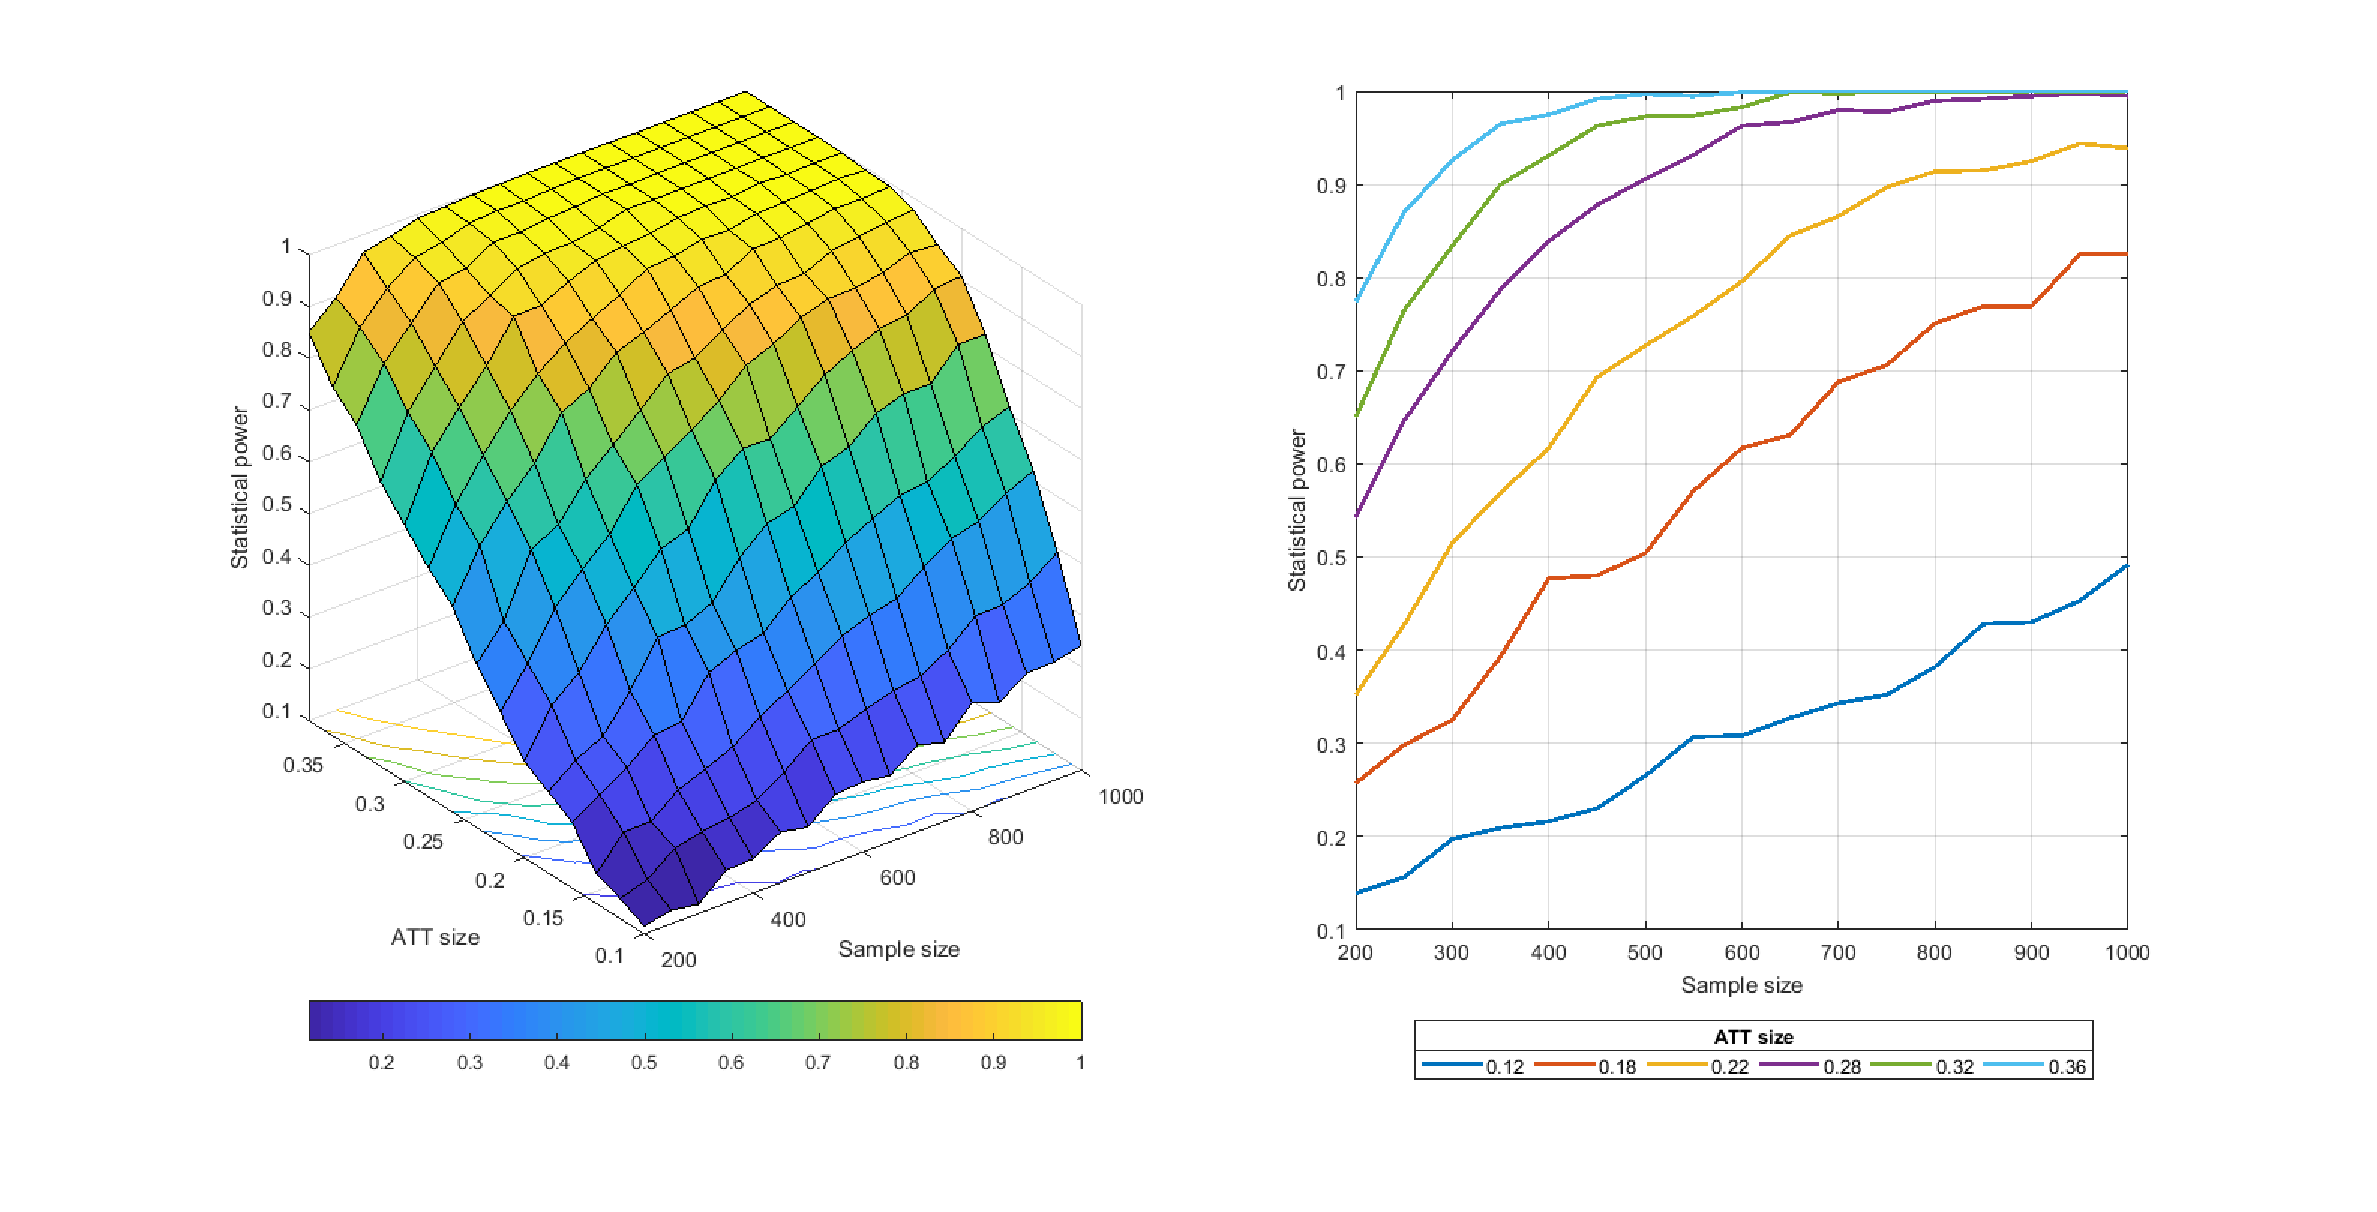
\includegraphics[width=0.75\textwidth]{Figuras/pwr_AB_FS_4.pdf}
        \end{center}
\end{figure}
    
{\footnotesize \textit{Do files: } \texttt{sim\_AB\_FS\_1.do, simulation\_iv.do}}    
    
\end{frame}

\section{Inferencia Causal}
\begin{frame}{Obervaciones Potenciales}

\onslide<1->{
    \[Y_i=\begin{cases}
Y_{1i}\quad \text{ if } D_i=1\\
Y_{0i}\quad \text{ if } D_i=0\end{cases}\]

\[Y_i=Y_{0i}+(Y_{1i}-Y_{0i})D_i\]


¿Cómo obtenemos efectos de tratamiento promedio - (ATE)? 
}

\onslide<2->{
\begin{align*}
    \mathbb{E}[Y_i\;|\;D_i=1, X_i]-&\mathbb{E}[Y_i\;|\;D_i=0, X_i] = \overbrace{\mathbb{E}[Y_{1i}\;|\;D_i=1, X_i]-\color{red}{\mathbb{E}[Y_{0i}\;|\;D_i=1, X_i]}}^{\text{ATT}}\\
    &+ \underbrace{\color{red}{\mathbb{E}[Y_{0i}\;|\;D_i=1, X_i]}-\color{black}\mathbb{E}[Y_{0i}\;|\;D_i=0, X_i]}_{\text{Bias}}
\end{align*}
}
\onslide<3->{
\center\emph{Problema fundamental de la inferencia causal}

\[\color{red}{\mathbb{E}[Y_{0i}\;|\;D_i=1, X_i]}\]
}
\end{frame}
\subsection{RCT}
\begin{frame}{RCT : $\lbrace Y_i\rbrace \perp (D_i\;|\; X_i)$}


\begin{table}[H]
    \caption{Treatment Effects}
    \begin{center}
    {\fontsize{4.5}{4.5}\selectfont{% Table generated by Excel2LaTeX from sheet 'treatment_effects'
\begin{tabular}{lcccccccc}
\toprule
\multicolumn{1}{|r}{} & \multicolumn{8}{c}{Months after treatment} \\
\midrule
\multicolumn{1}{r|}{} & \multicolumn{5}{c|}{Same day settlement} & \multicolumn{1}{c|}{2 months } & \multicolumn{1}{c|}{ 5 months} & Long run \\
\midrule
\midrule
\multicolumn{1}{r|}{} & \multicolumn{2}{c|}{Phase 1} & \multicolumn{2}{c|}{Phase 2} & \multicolumn{4}{c}{Phase 1/2} \\
\midrule
\multicolumn{1}{r|}{} & \multicolumn{5}{c|}{OLS}              & \multicolumn{3}{c|}{OLS} \\
\midrule
\midrule
      & (1)   & (2)   & (3)   & (4)   & (5)   & (6)   & (7)   & (8) \\
\midrule
\midrule
Control (constant) & 0.060*** & 0.034*** & 0.11*** & 0.10*** & 0.094*** & 0.15*** & 0.39*** & 0.45*** \\
      & (0.013) & (0.011) & (0.030) & (0.030) & (0.026) & (0.043) & (0.039) & (0.049) \\
Calculator & 0.051** & 0.019 & 0.047** & 0.0077 & 0.018 & 0.0035 & -0.0069 & -0.0025 \\
      & (0.022) & (0.019) & (0.021) & (0.019) & (0.014) & (0.021) & (0.024) & (0.025) \\
Conciliator & 0.054*** & 0.033* &       &       & 0.016 & -0.0028 & -0.030 & -0.053 \\
      & (0.019) & (0.018) &       &       & (0.019) & (0.023) & (0.028) & (0.036) \\
Emp present (EP) &       & 0.14*** &       & 0.14* & 0.14*** & 0.11** & 0.094* & 0.070 \\
      &       & (0.050) &       & (0.072) & (0.041) & (0.046) & (0.048) & (0.050) \\
Calculator\#EP &       & 0.16** &       & 0.16* & 0.16*** & 0.18*** & 0.16** & 0.14** \\
      &       & (0.079) &       & (0.089) & (0.056) & (0.061) & (0.064) & (0.061) \\
Conciliator\#EP &       & 0.16** &       &       & 0.16** & 0.21*** & 0.27*** & 0.20** \\
      &       & (0.074) &       &       & (0.071) & (0.079) & (0.075) & (0.078) \\
\midrule
Observations & 1074  & 1074  & 1092  & 1092  & 2166  & 2166  & 2166  & 2166 \\
R-squared & 0.0072 & 0.12  & 0.051 & 0.11  & 0.13  & 0.12  & 0.11  & 0.087 \\
Court dummies  & NO    & NO    & YES   & YES   & YES   & YES   & YES   & YES \\
DepVarMean & \multicolumn{2}{c}{0.095} & \multicolumn{2}{c}{0.20} & 0.15  & 0.19  & 0.32  & 0.43 \\
InteractionVarMean &       & 0.18  &       & \multicolumn{5}{c}{0.18} \\
Calc=Conc & 0.88  & 0.53  & -     & -     & 0.94  & 0.82  & 0.79  & 0.40 \\
Calc\#EP=Conc\#EP & -     & 0.98  & -     & -     & 1.00  & 0.58  & 0.68  & 0.085 \\
\bottomrule
\bottomrule
\end{tabular}%
}}
    \end{center}
\end{table}

\end{frame}

\subsection{IV - CF}

\begin{frame}{IV - corrigiendo la endogeneidad}

Consideremos un modelo $y_i = X_i\beta + \epsilon_i$

\[\hat\beta_{OLS} = (X'X)^{-1}X'y = (X'X)^{-1}X'(X\beta\epsilon) = \beta + (X'X)^{-1}X'\epsilon\]
\pause

\begin{block}{Variables instrumentales $Z$}
\begin{itemize}
    \item Primera etapa fuerte :  $ \quad X_i = Z_i\gamma+\nu_i$
    \item Restricción de exclusión : $\quad Z'e = 0$
\end{itemize}
\end{block}  

\pause
\[\hat\beta_{IV} = (Z'X)^{-1}Z'y\rightarrow \beta\]

\begin{block}{Estimación - 2SLS}
\begin{enumerate}[(i)]
    \item $X=Z\gamma+\nu$
    \[\hat\gamma = (Z'Z)^{-1}Z'X\]
    \[\hat X = X\hat\gamma = \underbrace{Z(Z'Z)^{-1}Z'}_{P_Z}X\]
    \item $y = \hat X\beta +\epsilon$
    \[\hat\beta_{2SLS} = (X'P_ZX)^{-1}X'P_zy= \hat\beta_{GMM}\]
\end{enumerate}
\end{block}
\end{frame}
\begin{frame}[label=inst]{¿Instrumentos?}
    \begin{itemize}
    \pause
        \item Lluvia \pause  - \color{red} no funcionó
    \pause
        \item \color{black}\hyperlink{dist}{\beamerbutton{Distancia}} a la junta \pause  - \color{red} no funcionó
    \end{itemize}
\end{frame}

\begin{frame}[allowframebreaks]{Control function}

Es un método de dos etapas \emph{generalizado}, pues explota la estructura de la variable endógena - por lo que obtenemos residuos generalizados.

\begin{align*}
    y = X\beta+\epsilon\quad\quad\quad &\text{ Ec. estructural}\\
    X = Z\gamma + \nu  \quad\quad\quad &\text{ Primera etapa}\\
    \mathbb{E}[Z'\nu]= 0 \quad\quad\quad &\text{ Ortogonalidad}\\
    \epsilon = \nu\rho + u \quad \quad \mathbb{E}[\nu u]=0 \quad\quad\quad &\text{ Residuo generalizado}
\end{align*}

De la última ecuación: $\color{red}\rho \color{black}=\mathbb{E}[\nu\nu']^{-1}\mathbb{E}[\nu\epsilon]$
y notemos que 
\[\lbrace\epsilon,\nu\rbrace \perp Z \Longrightarrow u\perp Z\]
\[ \therefore u\perp X\]
Entonces,
\begin{block}{CF}
 \[y = X\beta+\nu\rho + u\]
\end{block}

\framebreak

\begin{enumerate}
    \item En el modelo lineal básico con coeficientes constantes, donde las VEE aparecen linealmente, y donde uso formas reducidas lineales, CF es lo mismo que 2SLS. Pero el primero proporciona una prueba simple y robusta de la hipótesis nula de que $X$ es exógena : $\rho=0$
    \item Cuando exploto características especiales de la VEE, por ejemplo, reconozco que es una variable binaria, CF es probablemente más eficiente que 2SLS pero, en términos de consistencia, el enfoque de CF suele ser menos robusto que el de IV.
    \item  En modelos con múltiples funciones no lineales de VEE, el enfoque CF maneja parsimoniosamente la endogeneidad y proporciona pruebas de exogeneidad simples.
\end{enumerate}

\framebreak


\begin{figure}[H]
    \begin{center}
        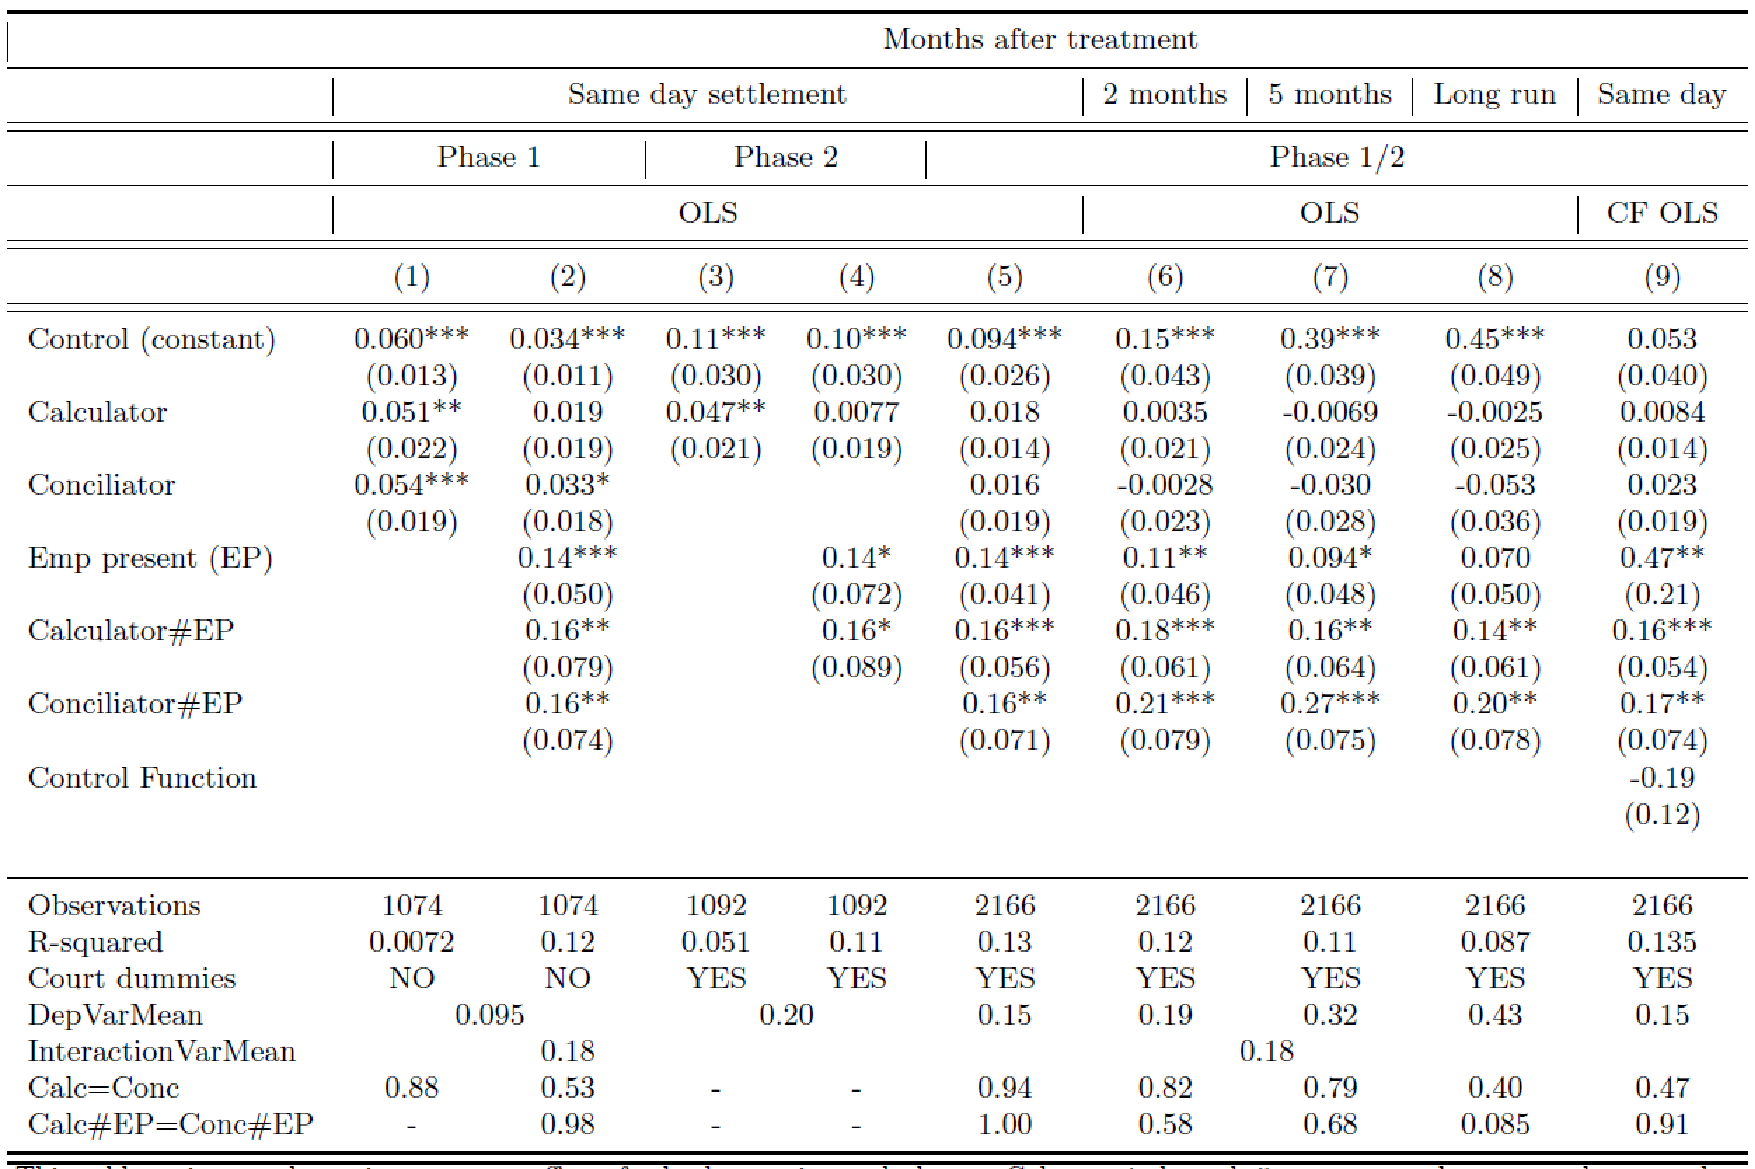
\includegraphics[width=0.8\textwidth]{Figuras/te.pdf}
        \end{center}
\end{figure}
    
{\footnotesize \textit{Do files: } \texttt{treatment\_effects.do, treatment\_effects\_IV\_CF.do}}  
\end{frame}



\subsection{Matching}
\begin{frame}{Matching}
    Recordemos el problema fundamental de inferencia causal: ¿$\mathbb{E}[Y_{0i}\;|\;D_i=1, X_i]$?
    
    \begin{block}{Supongamos : \emph{strong ignorability}}
     CIA : $(Y_i | X) \perp D_i$\\
     Overlap : $0<e(x):=\mathbb{E}[D_i\;|\;X_i=x]<1$ para todo $x$ en el soporte de $X$
    \end{block}
    \pause
    Sea 
    \[m(i) = \operatorname{argmin}_{j : D_j\neq D_i}||X_i-X_j||\]
    
    \begin{align*}
        \hat Y_i(0) = \begin{cases}
        Y_i^{obs} \;\;\text{ si } \;D_i=0\\
        Y_{m(i)}^{obs} \;\;\text{ si } \;D_i=1
        \end{cases}
        \;\;&\;\;
      \hat Y_i(1) = \begin{cases}
        Y_{m(i)}^{obs} \;\;\text{ si } \;D_i=0\\
        Y_i^{obs} \;\;\text{ si } \;D_i=1
        \end{cases}    \\
        \hat X_i(0) = \begin{cases}
        X_i^{obs} \;\;\text{ si } \;D_i=0\\
        X_{m(i)}^{obs} \;\;\text{ si } \;D_i=1
        \end{cases}
        \;\;&\;\;
      \hat X_i(1) = \begin{cases}
        X_{m(i)}^{obs} \;\;\text{ si } \;D_i=0\\
        X_i^{obs} \;\;\text{ si } \;D_i=1
        \end{cases}          
    \end{align*}
    
El estimador de matching está dado por:
\[\hat\tau=\frac{1}{N}\sum_{i}\hat Y_i(1)-\hat Y_i(0)\]

\pause
Se puede mejorar el sezgo de este estimador usando regresión lineal para \emph{ajustar el sezgo} asociado con diferencias entre $\hat X_i(0)$ y $\hat X_i(1)$.
\end{frame}

\begin{frame}[allowframebreaks]{Estimación}

(I) `Verificar' overlap - Trimming procedure\\
    
        \begin{figure}[H]
    \begin{center}
     \begin{subfigure}{0.4\textwidth}
    \caption*{No trimming}
            \centering
            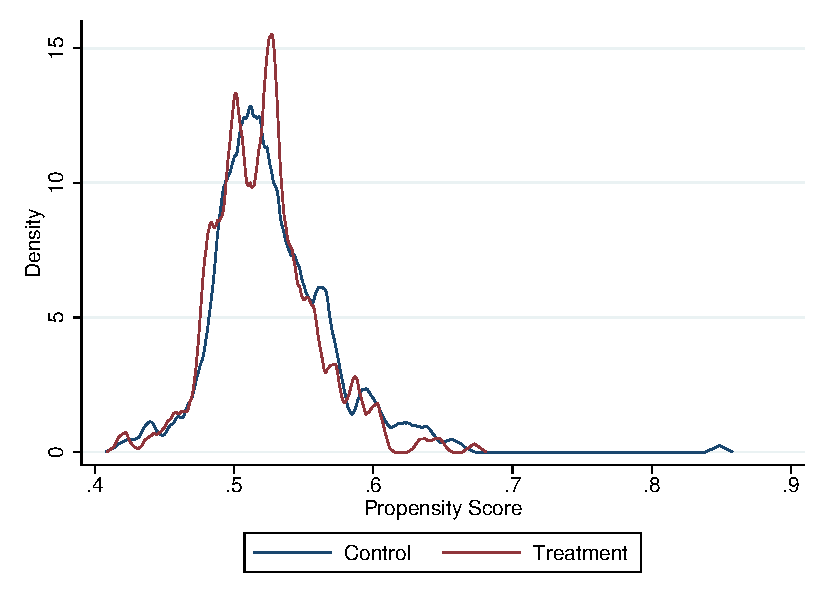
\includegraphics[width=\textwidth]{Figuras/ps_overlap_before.pdf}
        \end{subfigure}
             \begin{subfigure}{0.4\textwidth}
    \caption*{Trimming}
            \centering
            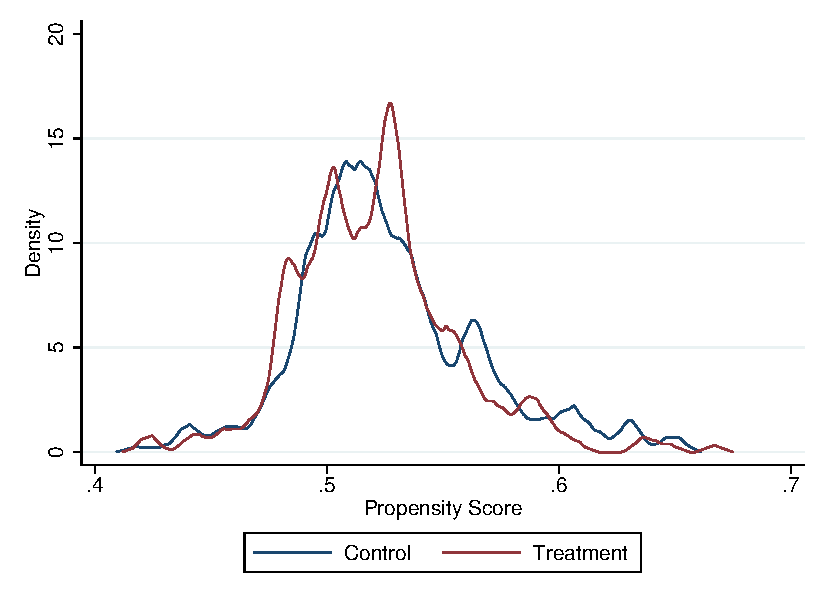
\includegraphics[width=\textwidth]{Figuras/ps_overlap.pdf}
        \end{subfigure}
    \end{center}
     {\footnotesize {$\hat e(x)= \frac{\exp{\beta'x}}{1+\beta'x}$}} 
\end{figure}

\framebreak
    
    
(II) Balance
\begin{table}[H]
    \caption{Balance}
    \begin{center}
    {\scriptsize{% Table generated by Excel2LaTeX from sheet 'balance_match'
\begin{tabular}{lccc}
\toprule
      & Control & Treatment & p-value \\
\midrule
\midrule
Entitlement by law & 60234.96 & 57567.95 & 0.62 \\
      & (3400.38) & (4098.63) &  \\
Public lawyer & 0.08  & 0.09  & 0.77 \\
      & (0.01) & (0.01) &  \\
Woman & 0.45  & 0.45  & 0.86 \\
      & (0.02) & (0.03) &  \\
At will worker & 0.07  & 0.06  & 0.44 \\
      & (0.01) & (0.01) &  \\
Tenure & 3.82  & 3.47  & 0.29 \\
      & (0.25) & (0.22) &  \\
Daily wage & 535.31 & 514.78 & 0.7 \\
      & (32.76) & (40.85) &  \\
Weekly hours & 58.5  & 56.79 & 0.12 \\
      & (0.81) & (0.73) &  \\
\midrule
Observations & 416   & 377   &  \\
\bottomrule
\bottomrule
\end{tabular}%
}}
    \end{center}
\end{table}

\framebreak
 (III) `Evaluar' CIA
\begin{table}[H]
    \caption{Pseudo-treatment effect}
    \begin{center}
    {\scriptsize{% Table generated by Excel2LaTeX from sheet 'unconfoundedness_match'
\begin{tabular}{lccc}
\toprule
\multicolumn{4}{c}{Pseudo treatment effect. Nearest-neighbor matching} \\
\midrule
\midrule
      & \multicolumn{3}{c}{Phase 1/2} \\
\midrule
\midrule
      & Entitlement & Daily wage & Tenure \\
\midrule
\midrule
      & (1)   & (2)   & (3) \\
\midrule
ATE   & 28.3  & -2.3  & -0.2 \\
      & (1162.4) & (11)  & (.2) \\
\% ATE & 0.05  & -0.43 & -5.22 \\
Baseline mean & 60342.9 & 536.2 & 3.8 \\
Obs   & \multicolumn{3}{c}{377} \\
Obs HD & \multicolumn{3}{c}{415} \\
Bias adjustment & YES   & YES   & YES \\
Matches & [1-3] & [1-3] & [1-3] \\
\bottomrule
\bottomrule
\end{tabular}%
}}
    \end{center}
\end{table}

\framebreak
 (III) Análisis
\begin{table}[H]
    \caption{Matching}
    \begin{center}
    {\scriptsize{% Table generated by Excel2LaTeX from sheet 'NN_match'
\begin{tabular}{lcccc|cc}
\toprule
\multicolumn{7}{c}{Treatment effect. Nearest-neighbor matching} \\
\midrule
\midrule
      & \multicolumn{6}{c}{Phase 1/2} \\
\midrule
\midrule
      & \multicolumn{4}{c|}{Variable matching} & \multicolumn{2}{c}{PSM} \\
\midrule
\midrule
      & (1)   & (2)   & (3)   & (4)   & (5)   & (6) \\
\midrule
ATE   & 2580  & 3536** & 3242* & 3939** & 3698* & 3995** \\
      & (1939) & (1715) & (1934) & (1725) & (1900) & (1554) \\
\% ATE & 34    & 47    & 43    & 52    & 49    & 53 \\
Baseline mean & \multicolumn{6}{c}{7598} \\
Obs   & \multicolumn{6}{c}{377} \\
Obs HD & \multicolumn{6}{c}{415} \\
Bias adjustment & NO    & NO    & YES   & YES   & -     & - \\
Matches & [1-1] & [1-3] & [1-1] & [1-3] & [1-1] & [1-3] \\
\bottomrule
\bottomrule
\end{tabular}%
}}
    \end{center}
\end{table}

{\footnotesize \textit{Do files: } \texttt{settlement\_conciliator\_matching.do}}  

\end{frame}


\subsection{Diff-in-Diff}
\begin{frame}{DiD - Parallel Worlds}
    \begin{tikzpicture}

% horizontal axis
\draw[->] (0,0) -- (7,0) node[anchor=north] ;
% labels
\draw	(2,0) node[anchor=north] {$T=0$}
		(6,0) node[anchor=north] {$T=1$};

\draw	(0,5) node[anchor=east] {$\mathbb{E}[Y_{1i,t=0}\,|\,D_i=1]$}
		(0,3) node[anchor=east] {$\mathbb{E}[Y_{1i,t=0}\,|\,D_i=1]$}
		(0,2) node[anchor=east] {$\mathbb{E}[Y_{0i,t=1}\,|\,D_i=0]$}
		(0,1) node[anchor=east] {$\mathbb{E}[Y_{0i,t=0}\,|\,D_i=0]$}
		;
		
		
% vertical axis
\draw[->] (0,0) -- (0,6) node[anchor=east];


\draw[thick] (2,1) -- (6,2) ;
\draw[thick] (2,3) -- (6,5) ;

\draw[dotted] (0,1) -- (2,1) ;
\draw[dotted] (0,3) -- (2,3) ;

\draw[dotted] (0,2) -- (6,2) ;
\draw[dotted] (0,5) -- (6,5) ;


\node at (2,1) [circle,fill,inner sep=1.5pt];
\node at (2,3) [circle,fill,inner sep=1.5pt];
\node at (6,2) [circle,fill,inner sep=1.5pt];
\node at (6,5) [circle,fill,inner sep=1.5pt];

\end{tikzpicture}
\end{frame}

\begin{frame}{DiD}
    \begin{tikzpicture}

% horizontal axis
\draw[->] (0,0) -- (7,0) node[anchor=north] ;
% labels
\draw	(2,0) node[anchor=north] {$T=0$}
		(6,0) node[anchor=north] {$T=1$};

\draw	(0,5) node[anchor=east] {$\mathbb{E}[Y_{1i,t=0}\,|\,D_i=1]$}
		(0,3) node[anchor=east] {$\mathbb{E}[Y_{1i,t=0}\,|\,D_i=1]$}
		(0,2) node[anchor=east] {$\mathbb{E}[Y_{0i,t=1}\,|\,D_i=0]$}
		(0,1) node[anchor=east] {$\mathbb{E}[Y_{0i,t=0}\,|\,D_i=0]$}
		;
		
		
% vertical axis
\draw[->] (0,0) -- (0,6) node[anchor=east];


\draw[thick] (2,1) -- (6,2) ;
\draw[thick] (2,3) -- (6,5) ;

\draw[dotted] (0,1) -- (2,1) ;
\draw[dotted] (0,3) -- (2,3) ;

\draw[dotted] (0,2) -- (6,2) ;
\draw[dotted] (0,5) -- (6,5) ;

\draw[dashed] (2,3) -- (6,4);

\node at (2,1) [circle,fill,inner sep=1.5pt];
\node at (2,3) [circle,fill,inner sep=1.5pt];
\node at (6,2) [circle,fill,inner sep=1.5pt];
\node at (6,5) [circle,fill,inner sep=1.5pt];
\node at (6,4) [circle,draw=black,fill=white,inner sep=1.5pt];

\end{tikzpicture}
\end{frame}

\begin{frame}{DiD}
    \begin{tikzpicture}

% horizontal axis
\draw[->] (0,0) -- (7,0) node[anchor=north] ;
% labels
\draw	(2,0) node[anchor=north] {$T=0$}
		(6,0) node[anchor=north] {$T=1$};

\draw	(0,5) node[anchor=east] {$\mathbb{E}[Y_{1i,t=0}\,|\,D_i=1]$}
		(0,4) node[anchor=east] {$\color{red}\mathbb{E}[Y_{0i,t=0}\,|\,D_i=1]$}
		(0,3) node[anchor=east] {$\mathbb{E}[Y_{1i,t=0}\,|\,D_i=1]$}
		(0,2) node[anchor=east] {$\mathbb{E}[Y_{0i,t=1}\,|\,D_i=0]$}
		(0,1) node[anchor=east] {$\mathbb{E}[Y_{0i,t=0}\,|\,D_i=0]$}
		;
		
		
% vertical axis
\draw[->] (0,0) -- (0,6) node[anchor=east];


\draw[thick] (2,1) -- (6,2) ;
\draw[thick] (2,3) -- (6,5) ;

\draw[dotted] (0,1) -- (2,1) ;
\draw[dotted] (0,3) -- (2,3) ;

\draw[dotted] (0,2) -- (6,2) ;
\draw[dotted] (0,5) -- (6,5) ;
\draw[dotted] (0,4) -- (6,4) ;


\draw[dashed] (2,3) -- (6,4);

\node at (2,1) [circle,fill,inner sep=1.5pt];
\node at (2,3) [circle,fill,inner sep=1.5pt];
\node at (6,2) [circle,fill,inner sep=1.5pt];
\node at (6,5) [circle,fill,inner sep=1.5pt];
\node at (6,4) [circle,draw=black,fill=white,inner sep=1.5pt];


\draw (6,4) -- (6,5) node [black,midway,anchor=west]{ATT}


\end{tikzpicture}
\end{frame}

\begin{frame}[label=did]{Impuesto a bebidas azucaradas}

Regresión DiD con FE: 

\begin{align*}
    C_{it}^{k} = \alpha_i+\gamma_t+\sum_{j=-12}^{12}\beta_k T_i\times I(t=j)+\nu_{it}
\end{align*}

donde $T_i=1$ si $i$ está en el grupo  \hyperlink{exposed_group}{\beamerbutton{más expuesto}}

    \begin{figure}[H]
    \begin{center}
        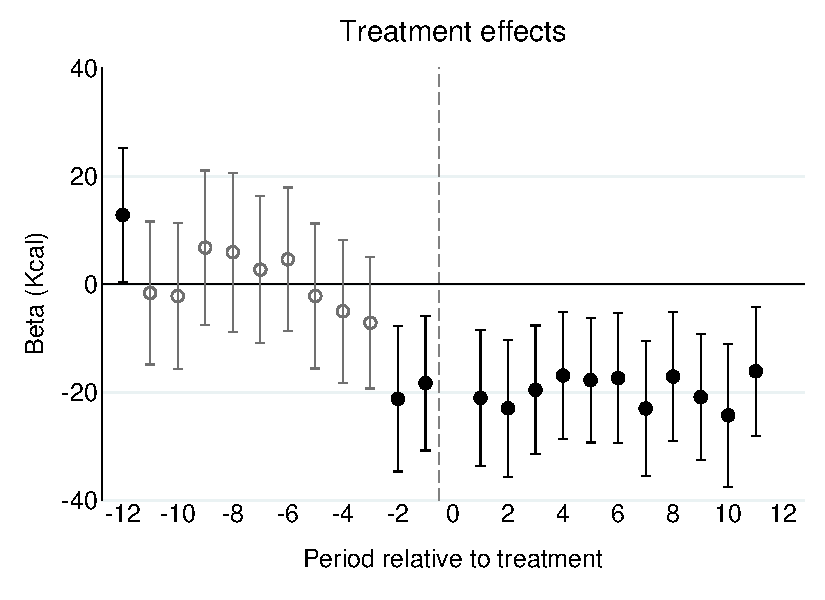
\includegraphics[width=0.7\textwidth]{Figuras/betas_did_sd_kcal_2_1.pdf}
        \end{center}
    {\footnotesize \textit{Do files: } \texttt{betas\_coef\_did.do}}    
          
\end{figure}

\end{frame}
\subsection{SCM}
\begin{frame}[allowframebreaks]{Synthetic Control Methods (SCM)}

Sean $(y_{tn}^0, y_{tn}^1)$ las observaciones potenciales para la unidad $n$ al tiempo $t$.

\[y_{tn}=D_{tn}y_{tn}^1+(1-D_{tn})y_{tn}^0 \;,\quad\quad D_{tn}=\begin{cases}
1\quad \text{ if } t\geq T_0, n=0\\
0\quad\text{ otherwise }
\end{cases}
\]

El efecto de tratamiento es :  $\tau_{tn}\equiv y_{tn}^1-y_{tn}^0$ \\


El supuesto clave en SCM es:

\begin{block}{}
Existen pesos $\beta_n\in[0,1]$ para $n=1,\ldots, N$ tales que
\[y_{t0}^0=\sum_{n=1}^N\beta_{n}y_{tn}^0\]
para $t=1\ldots, T$;y los pesos suman uno: $\sum_{n=1}^{N}\beta_n=1$.
\end{block}

El estimador en $t=T_0,\ldots, T$ está dado por:
\[\tau_t=y_{t0}^1-\sum_{n=1}^N\beta_{n}y_{t0}^0\]

\framebreak

Denotando por $x_t\equiv (y_{t1},\ldots,y_{tN})^\mathsf{T}$ a el vector de las observaciones para los controles. Podemos considerar el modelo de regresión

\begin{align}
\label{reg_model}
    y_{t0}=\beta^{\mathsf{T}}x_t+u_{t0}\quad\quad\quad t=1,\ldots, T_0
\end{align}

y la estimación por lo tanto está dada por:

\begin{align}
\label{adh}
   \operatorname{min} & \sum_{t=1}^{T_0}(y_{t0}-\beta^{\mathsf{T}}x_t)^2\\
    s.t. \quad & \nonumber \\
    & ||\beta||_1=1 \nonumber \\
    &\beta_i\geq 0\;\;\; i=1,\ldots, n \nonumber
\end{align}


\end{frame}

\begin{frame}{¿Inferencia?}
    
El principal problema con esta metodología es la dificultad para conducir \textbf{inferencia}, es decir, hay poco o ningún conocimiento sobre la distribución asintótica del estimador SCM, o su \textbf{intervalo de confianza}.\\



\begin{enumerate} [(i)]

    \item \emph{Enfoques de población finita} : Supuesto de que las unidades de tratamiento se asignan aleatoriamente y usan placebos, pruebas de permutación o alguna variante que explota la estructura de datos del panel, para realizar inferencia, que son llamados \\
    
    
    \item \emph{Enfoques asintóticos} : Los supuestos clave hacen que el número de individuos o períodos de tiempo tienden a infinito.
\end{enumerate}
\end{frame}

\begin{frame}{¿Inferencia?}
    
\begin{columns}

\begin{column}{0.5\textwidth}
\begin{figure}[H]
    \begin{center}
        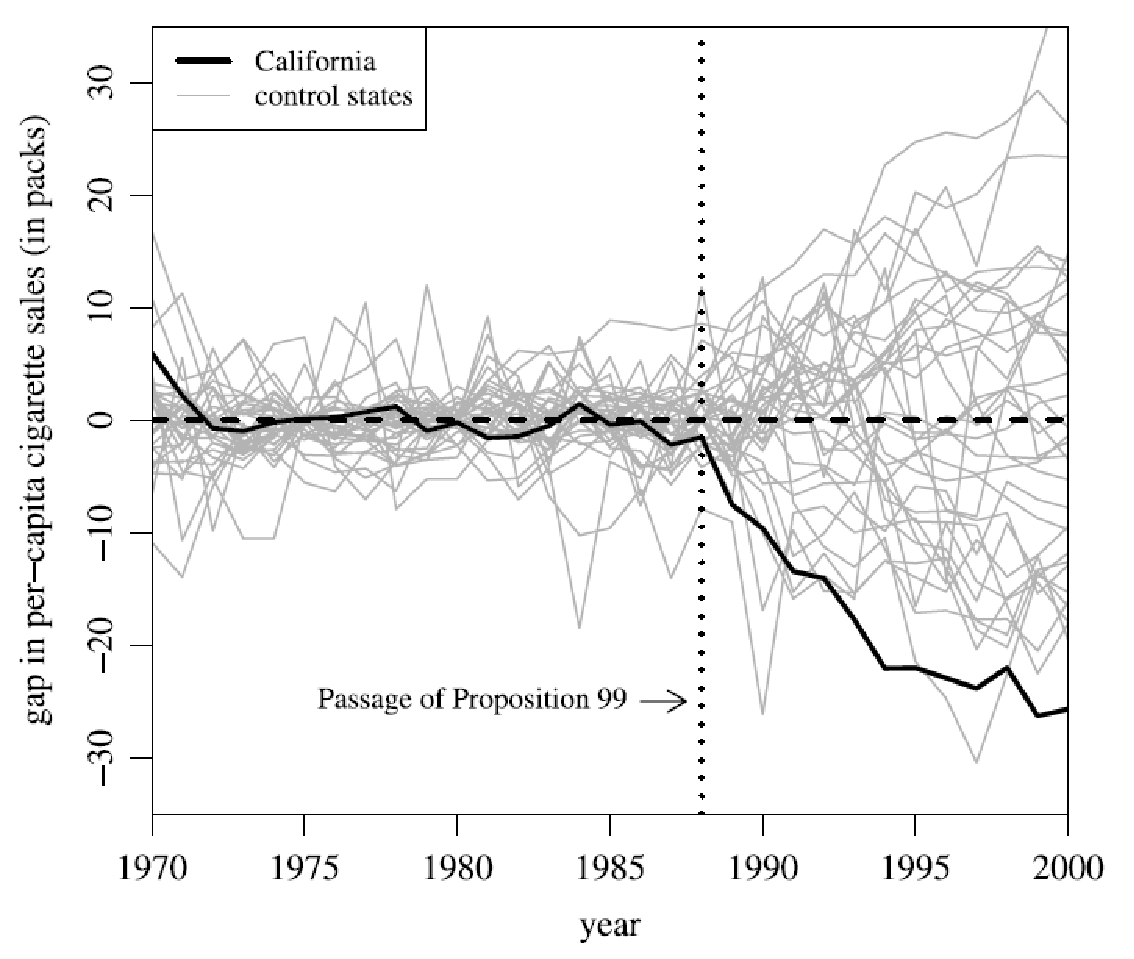
\includegraphics[width=0.95\textwidth]{Figuras/sc_adh.pdf}
        \end{center}
\end{figure}
\end{column}

\begin{column}{0.5\textwidth}

\end{column}

\end{columns}
\end{frame}

\begin{frame}{¡Inferencia!}
    
\begin{columns}

\begin{column}{0.5\textwidth}
\begin{figure}[H]
    \begin{center}
        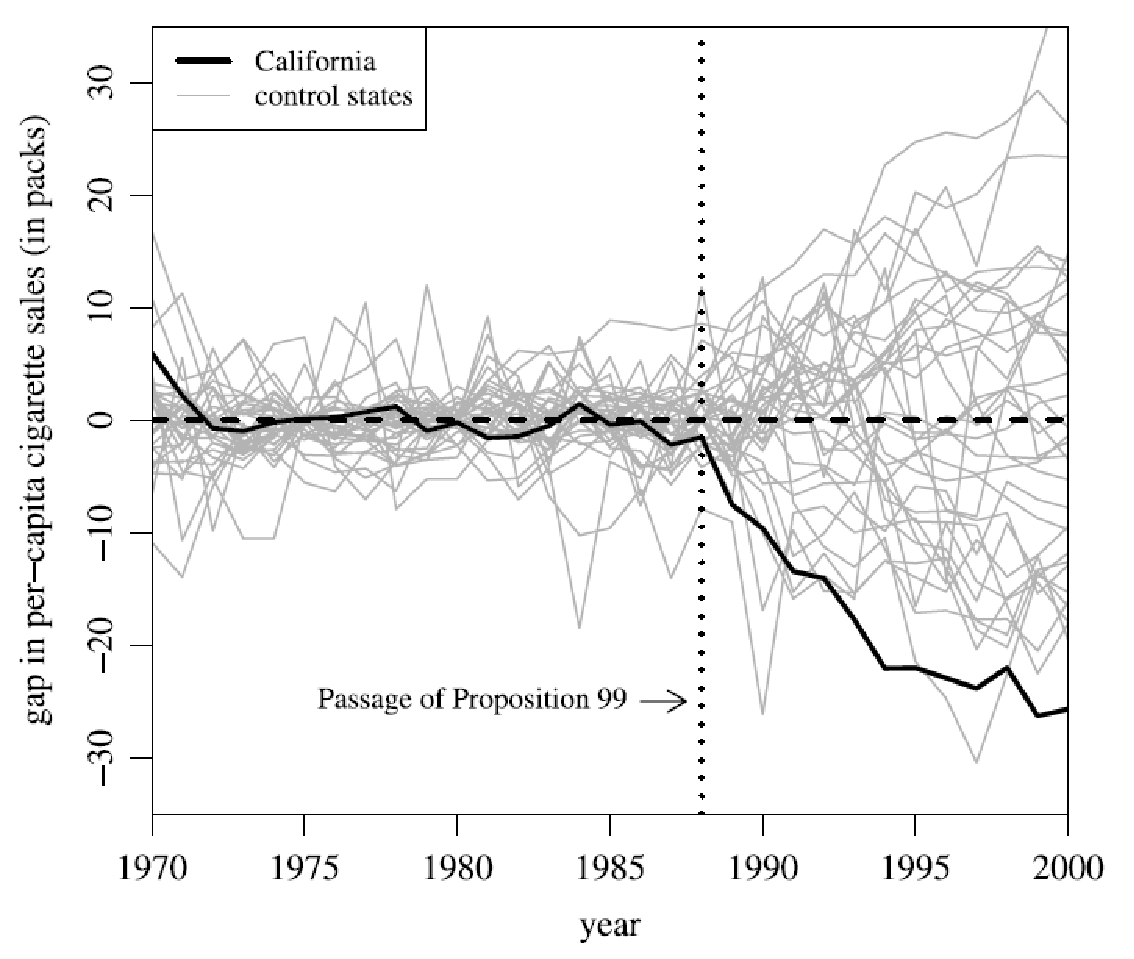
\includegraphics[width=0.95\textwidth]{Figuras/sc_adh.pdf}
        \end{center}
\end{figure}
\end{column}

\begin{column}{0.5\textwidth}
\animategraphics[autoplay,loop,height=5.0cm]{1}{ci_}{1}{3}
\end{column}

\end{columns}
\end{frame}

\begin{frame}{RWP}
    \begin{theorem}
    La región de confianza para el estimador SCM está dada por:
     \[B\left(\hat\tau_t,\mathsf{r}||x_t||+\sigma z_{(1-\alpha/2)}\right)\]
donde $\mathsf{r}=\frac{||\nabla R_{T_0}(\hat\beta)||+\sqrt{||\nabla R_{T_0}(\hat\beta)||^2-2|\Omega_{\hat\beta} |\left(R_{T_0}(\hat\beta)-T_0^{-1}\chi_{1-\alpha}\right)}}{|\Omega_{\hat\beta} |}$
    \end{theorem}
\end{frame}
\begin{frame}{SCM con datos panel}
Explotamos la estructura de panel y las múltiples unidades tratadas.
\pause
\begin{figure}[H]
    \begin{center}
        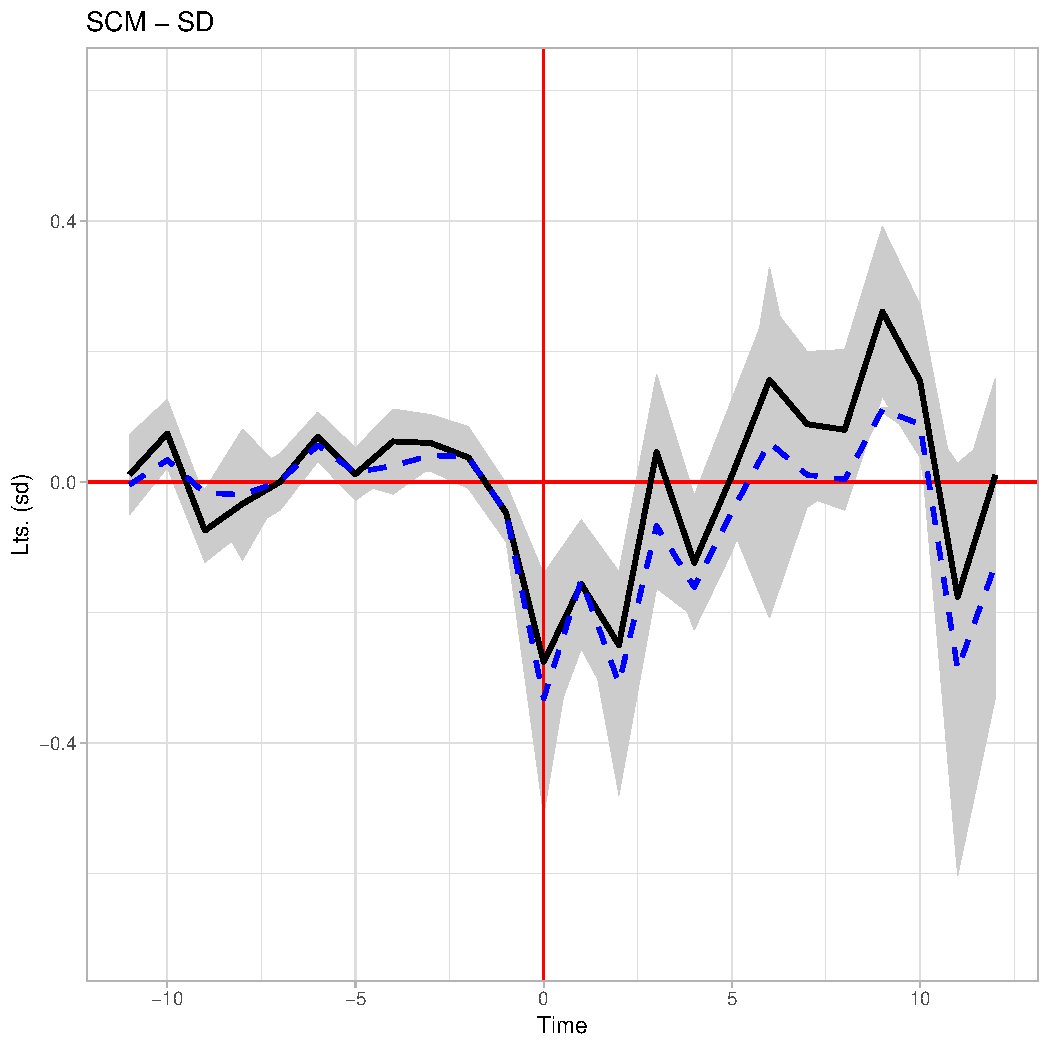
\includegraphics[width=0.5\textwidth]{Figuras/SD_scm_smooth_99.pdf}
        \end{center}
\end{figure}
 \textit{Rscript: } \texttt{SCM\_synth.R}
    

    
\end{frame}

\section{Attrition}

\subsection{Manski bounds}
\begin{frame}[allowframebreaks]{Manski bounds}
    \begin{itemize}
        \item Ningún supuesto sobre el mecanismo de selección
        \item La variable dependiente necesita estar acotada
        \item NA imputados de acuerdo al mínimo y máximo valor posible
        \item Cotas no informativas :(
    \end{itemize}
    
\framebreak

Sea $S_i$ una dummy identificando a los `no-attriters'.\\


\[\color{red}\text{¿}E[Y_{1i}\;|\;S_i = 0|D_i = 1]\quad\quad E[Y_{0i}\;|\;S_i = 0, D_i = 0]?\]

Worst-case scenario :  $E[Y_{1i}\;|\;S_i = 0|D_i = 1] = 0$ y $E[Y_{0i}\;|\;S_i = 0, D_i = 0] = 1$ \\


\begin{align*}
MB^{L} &= P(S_i = 1\;|\;D_i = 1)E(Y_i\;|\;D_i = 1, S_i = 1) \\
&- [P(S_i = 1\;|\;D_i = 0)E(Y_i\;|\;D_i = 0, S_i = 1) + P(S_i = 0\;|\;D_i = 0)]
\end{align*}

análogamente:

\begin{align*}
MB^{U} &= P(S_i = 1\;|\;D_i = 1)E(Y_i\;|\;D_i = 1, S_i = 1) + P(S_i = 0 \;|\; D_i = 1) \\
&- P(S_i = 1\;|\;D_i = 0)E(Y_i\;|\;D_i = 0, S_i = 1)
\end{align*}
\end{frame}

\subsection{Lee bounds}


\begin{frame}[allowframebreaks]{Lee bounds}
    
    \begin{itemize}
        \item RAT : $(Y_i, S_i) \perp D_i$
        \item Monotonicidad : $Pr(S_1\geq S_0)=1$
        
        Asignación de tratamiento sólo afecta \emph{attrition} en una dirección solamente.
    \end{itemize}

El objetivo es encontrar cotas 

\[LB^{L} \leq \mathbb{E}[Y_{1}-Y_{0}\;|\;S_0=1,S_1=1]\leq LB^{U}\]

\framebreak

\begin{theorem}
 Bajo RAT, monotonicidad y $PR(S=1\;|\;D=0)\neq 0$
\[LB^{L} = \mathbb{E}[Y\;|\;D=1, S=1, Y\leq F^{-1}(1-p)]-\mathbb{E}[Y\;|\;D=0, S=1]\]
\[LB^{U} = \mathbb{E}[Y\;|\;D=1, S=1, Y\geq F^{-1}(p)]-\mathbb{E}[Y\;|\;D=0, S=1]\]

donde $p=\frac{Pr(S=1\;|\;D=1)-Pr(S=1\;|\;D=0)}{Pr(S=1\;|\;D=1)}$.
\end{theorem}

\framebreak
\begin{figure}[H]
    \begin{center}
        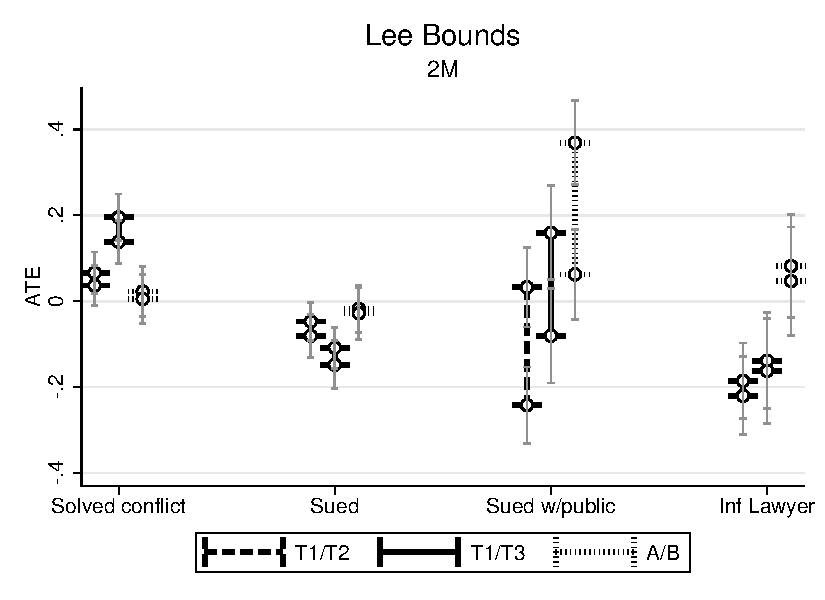
\includegraphics[width=0.7\textwidth]{Figuras/lee_bounds_2m.pdf}
        \end{center}
\end{figure}
 \textit{Do files: } \texttt{plot\_lee\_bounds.do}
    
\end{frame}
\section{Clasificación}
%Quality of lawyers
\begin{frame}{Calificación de abogados}
    \begin{table}[H]
\caption{Predicciones}
\begin{center}
\tiny{% Table generated by Excel2LaTeX from sheet 'prediction_lawyer_accuracy'
\begin{tabular}{rccccccccc}
\toprule
      & Outcome & \multicolumn{2}{c}{Judge ruling prediction} & \multicolumn{2}{c}{End mode prediction} & \multicolumn{2}{c}{Payment prediction} & \multicolumn{2}{c}{Total} \\
\midrule
\midrule
      & Lawyer & Lawyer & Calc  & Lawyer & Calc  & Lawyer & Calc  & Lawyer & Calc \\
\midrule
\midrule
1     & 12.8\% & 44.4\% & \cellcolor[rgb]{ .929,  .929,  .929} 27.8\% & 61.1\% & \cellcolor[rgb]{ .929,  .929,  .929} 55.6\% & 19.5\% & \cellcolor[rgb]{ .929,  .929,  .929} 19.5\% & 34.5\% & \cellcolor[rgb]{ .929,  .929,  .929} 34.3\% \\
2     & 11.2\% & 62.5\% & \cellcolor[rgb]{ .929,  .929,  .929} 68.8\% & 87.5\% & \cellcolor[rgb]{ .929,  .929,  .929} 62.5\% & 0\%   & \cellcolor[rgb]{ .929,  .929,  .929} 12.8\% & 40.3\% & \cellcolor[rgb]{ .929,  .929,  .929} 48\% \\
3     & 15.2\% & 56.3\% & \cellcolor[rgb]{ .929,  .929,  .929} 62.5\% & 62.5\% & \cellcolor[rgb]{ .929,  .929,  .929} 62.5\% & 22.7\% & \cellcolor[rgb]{ .929,  .929,  .929} 17.3\% & 39.2\% & \cellcolor[rgb]{ .929,  .929,  .929} 47.4\% \\
4     & 35.2\% & 45.5\% & \cellcolor[rgb]{ .929,  .929,  .929} 50\% & 36.4\% & \cellcolor[rgb]{ .929,  .929,  .929} 77.3\% & 15.3\% & \cellcolor[rgb]{ .929,  .929,  .929} 18.8\% & 33.1\% & \cellcolor[rgb]{ .929,  .929,  .929} 48.7\% \\
5     & 5.6\% & 33.3\% & \cellcolor[rgb]{ .929,  .929,  .929} 75\% & 33.3\% & \cellcolor[rgb]{ .929,  .929,  .929} 62.5\% & 9.9\% & \cellcolor[rgb]{ .929,  .929,  .929} 19.8\% & 20.5\% & \cellcolor[rgb]{ .929,  .929,  .929} 52.4\% \\
6     & 9.6\% & 60\%  & \cellcolor[rgb]{ .929,  .929,  .929} 70\% & 70\%  & \cellcolor[rgb]{ .929,  .929,  .929} 65\% & 0\%   & \cellcolor[rgb]{ .929,  .929,  .929} 18.6\% & 34.9\% & \cellcolor[rgb]{ .929,  .929,  .929} 51.2\% \\
7     & 16\%  & 50\%  & \cellcolor[rgb]{ .929,  .929,  .929} 55.6\% & 55.6\% & \cellcolor[rgb]{ .929,  .929,  .929} 72.2\% & 13.9\% & \cellcolor[rgb]{ .929,  .929,  .929} 13.9\% & 33.9\% & \cellcolor[rgb]{ .929,  .929,  .929} 47.2\% \\
8     & 13.6\% & 54.5\% & \cellcolor[rgb]{ .929,  .929,  .929} 77.3\% & 86.4\% & \cellcolor[rgb]{ .929,  .929,  .929} 72.7\% & 21.4\% & \cellcolor[rgb]{ .929,  .929,  .929} 21.4\% & 44\%  & \cellcolor[rgb]{ .929,  .929,  .929} 57.1\% \\
\bottomrule
\bottomrule
\end{tabular}%
}
\end{center}
    
    {\footnotesize \textit{Do files: } \texttt{lawyer\_dataset.do, lawyer\_dataset\_predicc.do, cleaning\_base\_calidad.do, calif\_abogados\_pagos.do}} 
    
\end{table}
\end{frame}

\subsection{Gráficas de heterogeneidad por efectos fijos}
\begin{frame}[allowframebreaks]{Heterogeneidad - FE}
           \begin{figure}[H]
\caption{Heterogeneous outcome graphs}
    \begin{center}
     \begin{subfigure}{0.25\textwidth}
    \caption*{\% Positive recovery}
            \centering
            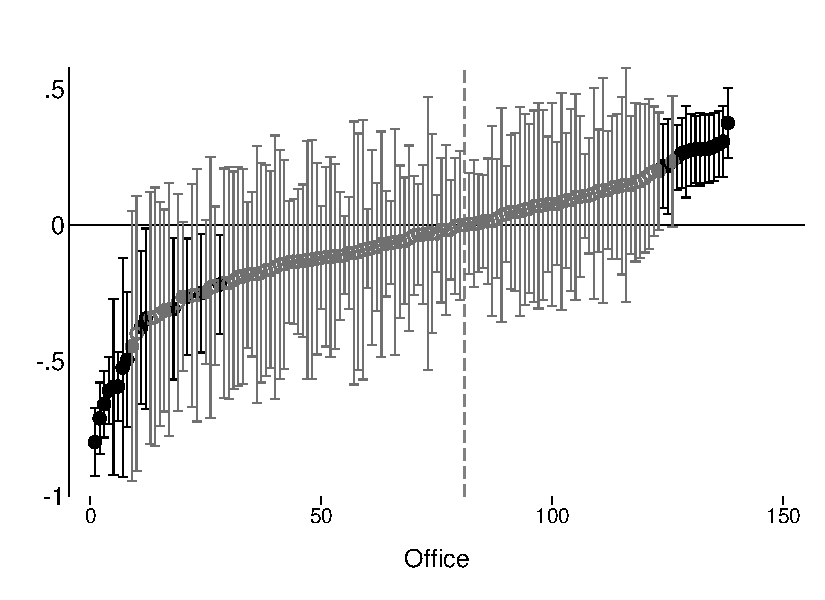
\includegraphics[width=\textwidth]{Figuras/betas_pos_rec.pdf}
        \end{subfigure}
                \begin{subfigure}{0.25\textwidth}
            \caption*{Win/Entitlement}
            \centering
            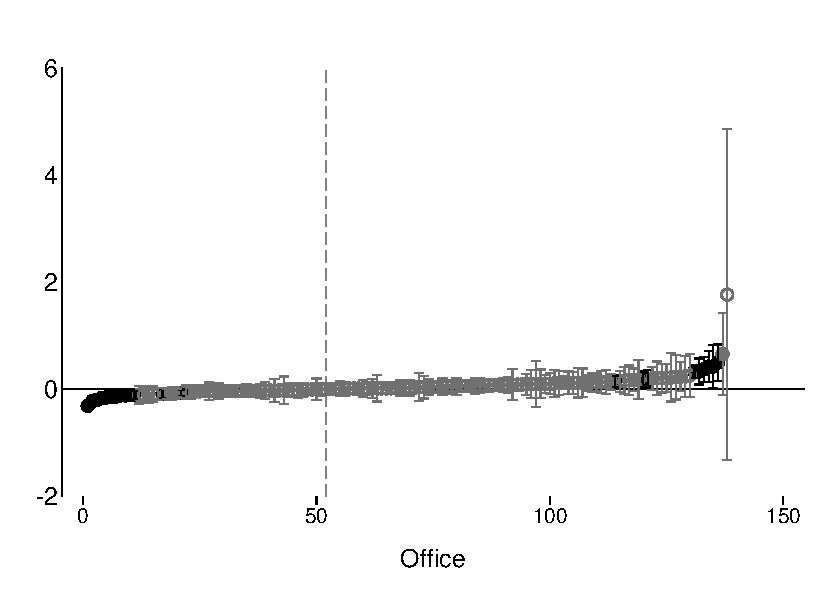
\includegraphics[width=\textwidth]{Figuras/betas_win_minley.pdf}
        \end{subfigure}
                \begin{subfigure}{0.25\textwidth}
            \caption*{Duration}
            \centering
            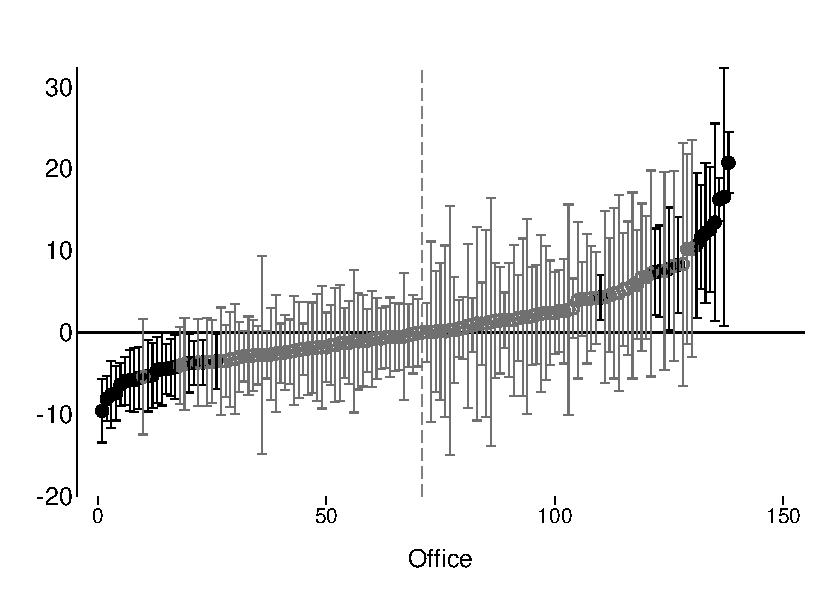
\includegraphics[width=\textwidth]{Figuras/betas_duration.pdf}
        \end{subfigure}
             \begin{subfigure}{0.25\textwidth}
    \caption*{(Office)}
            \centering
            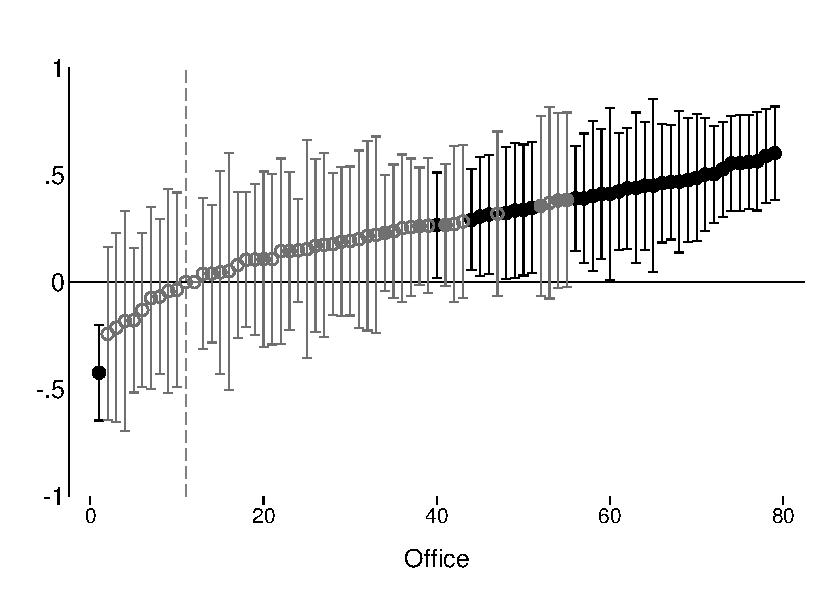
\includegraphics[width=\textwidth]{Figuras/betas_desp_pos_rec.pdf}
        \end{subfigure}        
     \begin{subfigure}{0.25\textwidth}
            \caption*{(Office)}
            \centering
            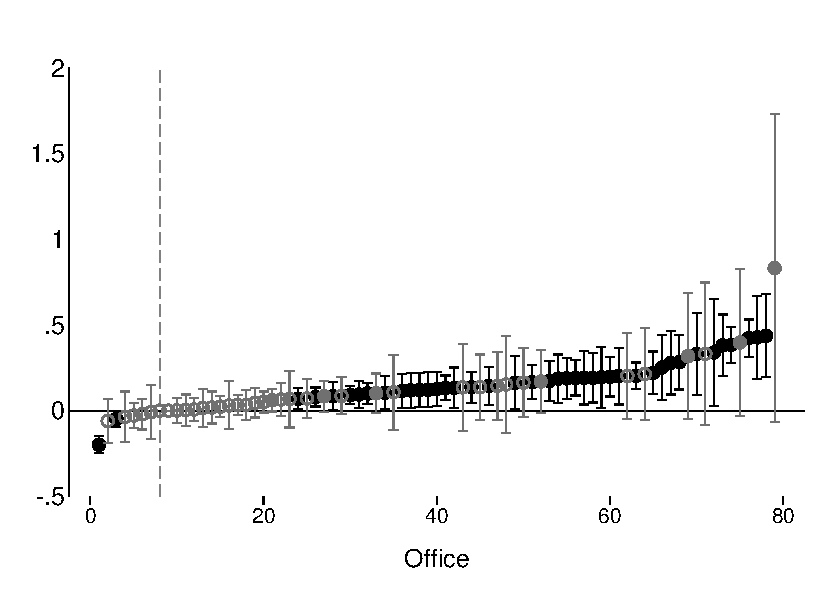
\includegraphics[width=\textwidth]{Figuras/betas_desp_win_minley.pdf}
        \end{subfigure}
         \begin{subfigure}{0.25\textwidth}
            \caption*{(office)}
            \centering
            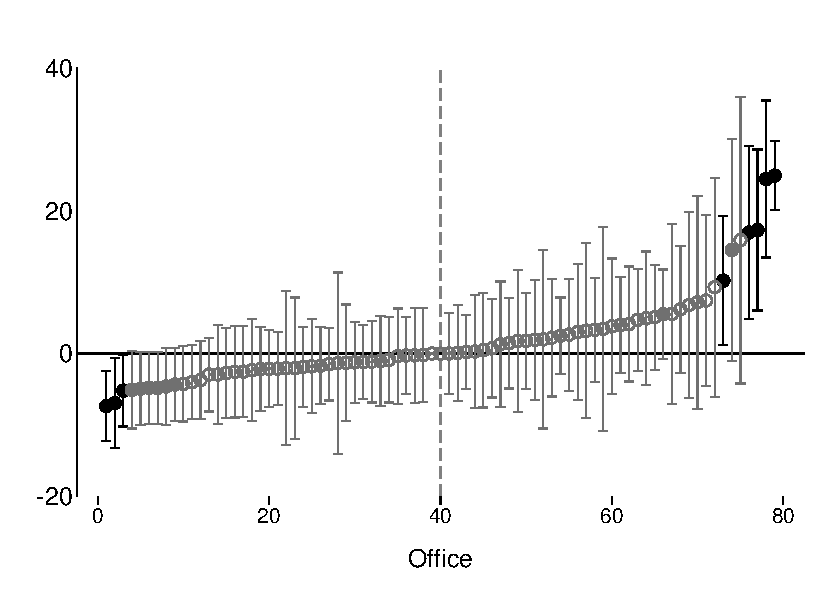
\includegraphics[width=\textwidth]{Figuras/betas_desp_duration.pdf}
        \end{subfigure}
    \end{center}
 \footnotesize
 \textit{Do files: } \texttt{fe\_betas\_pres.do, fe\_betas\_desp.do}
\end{figure}

    
\end{frame}



\subsection{Clustering  \&  PCA}
\begin{frame}{Clusters : Buenos/Malos}
    \begin{figure}[H]
    \begin{center}
        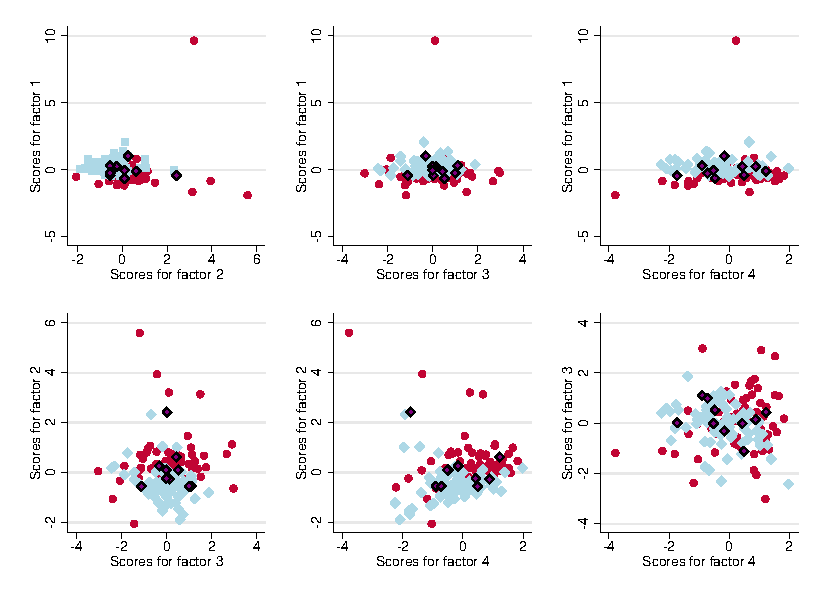
\includegraphics[width=0.7\textwidth]{Figuras/cluster_2.pdf}
        \end{center}
\end{figure}
 \textit{Do files: } \texttt{lawyer\_dataset\_collapsed.do, cluster\_analysis.do}
\end{frame}

\begin{frame}{Gracias :)}
    
\end{frame}

\appendix
\begin{frame}[label=dist]{Instalación de OSRM}

\begin{enumerate}[(1)]
    \item Install \color{blue}\href{https://nodejs.org/en/}{Node.js} \color{black} 8.11.3 LTS (or current)
    \item Extract the file osrm\_Release.zip (link from my \color{blue}\href{https://www.dropbox.com/s/eeo5f9ws7hmair4/osrm_Release.zip?dl=0}{Dropbox}).\color{black} This is the latest OSRM Windows build.
    \item \color{black} Copy the file  \color{blue}\href{https://download.geofabrik.de/north-america/mexico-latest.osm.pbf}{mexico-latest.osm.pbf} \color{black}in the osrm\_Release folder.
    \item Open Node.js command prompt
   \begin{enumerate}
        \item Change directory to the osrm\_Release folder\\
        
                \texttt{         cd $\sim$/osrm\_Release}  
                
        \item Extracting the road network\footnote{If instead you want MLD use \texttt{osrm-partition} and \texttt{osrm-customize} instead of \texttt{osrm-contract}.}\\
        
                \texttt{         osrm-extract mexico-latest.osm.pbf}
                
                \texttt{         osrm-contract mexico-latest.osm.pbf}
            
    \end{enumerate}
\end{enumerate}

This previous steps only need to be done once. This sets the road network for Mexico.
    \begin{itemize}
        \item You can also download the road network files \color{blue}\href{https://www.dropbox.com/s/2yflj2kfb24ujms/mexico-latest.zip?dl=0}{here}. \color{black} (Extract and copy in the osrm-Release folder.) 
    \end{itemize}
    
    \begin{enumerate}[(1)]
\setcounter{enumi}{4}
\item Install R package \texttt{osrm} - (Version I'm using is \textbf{\texttt{\href{https://cran.r-project.org/src/contrib/Archive/osrm/}{Package} osrm version 3.0.2}})
    \end{enumerate}
    
\end{frame}
\begin{frame}[allowframebreaks]{Instalación de OSRM}
    
In order to launch OSRM as a local instance the following steps are needed.
    \begin{enumerate}
        \item Change directory to the osrm\_Release folder in  Node.js command prompt\\
        
        \texttt{         cd $\sim$/osrm\_Release}
        \textcolor{white}{      cd C:/Users/xps-seira/Dropbox/repos/osrm/osrm-backend      }

        \item Set the local OSRM instance\\
        
        \texttt{         osrm-routed --max-table-size=1500 mexico-latest.osrm }
        \item In R, run the script:
    \end{enumerate}
    
\lstinputlisting{./Rscripts/geocode.R}

\framebreak


\begin{figure}[H]
    \begin{center}
        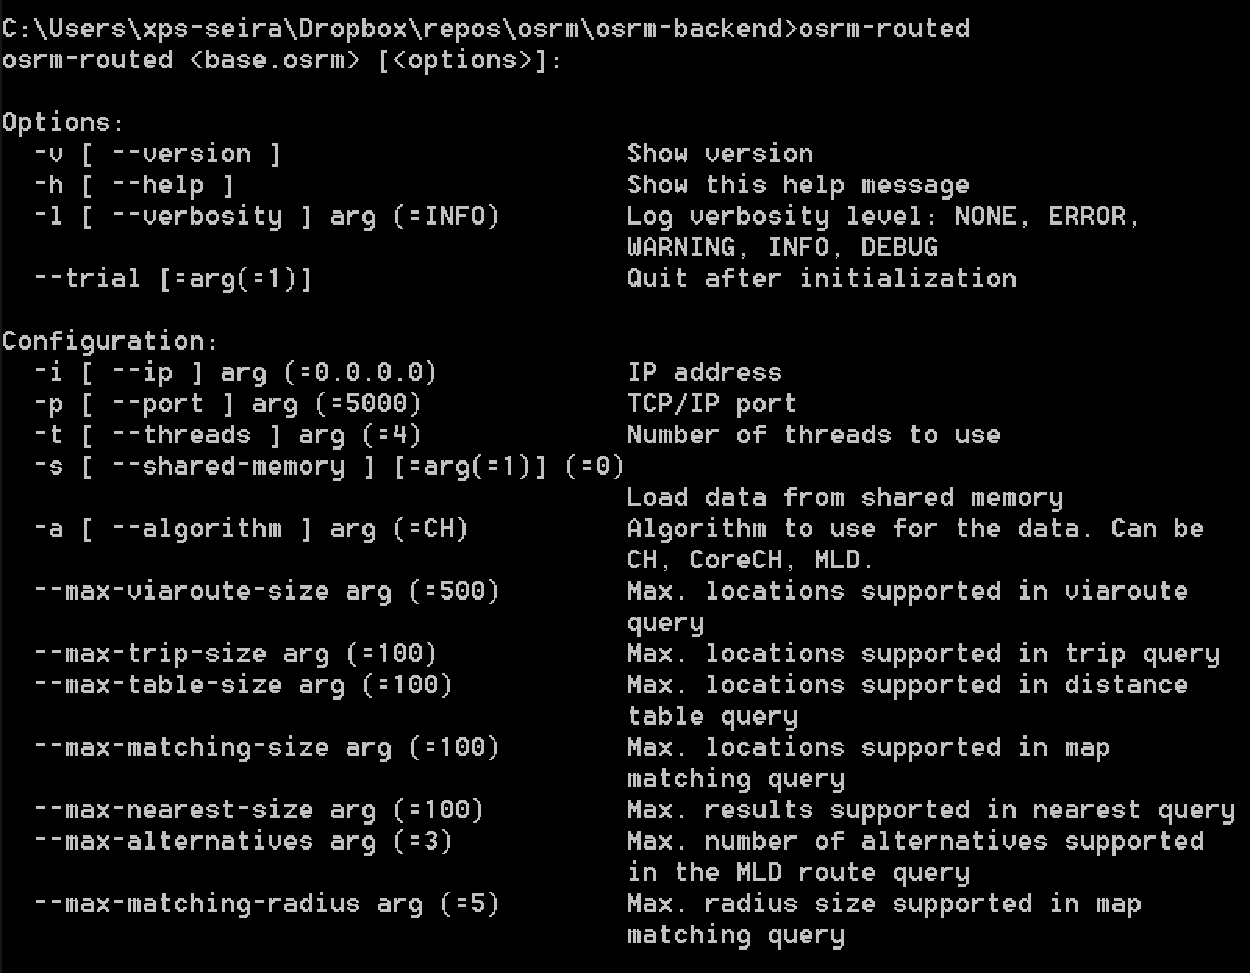
\includegraphics[width=0.7\textwidth]{Figuras/osrm.pdf}
        \end{center}
\end{figure}
\end{frame}

\begin{frame}{Recursos}
\begin{itemize}
    \item Github repo : \href{https://github.com/Project-OSRM/osrm-backend}{https://github.com/Project-OSRM/osrm-backend}
    \item Build using docker on Windows : \href{https://phabi.ch/2020/05/06/run-osrm-in-docker-on-windows/}{https://phabi.ch/2020/05/06/run-osrm-in-docker-on-windows/}
\end{itemize}

\vspace{35mm}
De regreso a los \hyperlink{inst}{\beamerbutton{instrumentos}}.

\end{frame}

\begin{frame}[label=exposed_group]{Definición de grupo expuesto}

Definir un grupo de tratamiento / control puro. Lo haremos eligiendo una partición óptima de la distribución total del gasto sujeto a impuestos, ya que es probable que los grandes gastadores sean más sensibles a un cambio de precio en SD, por lo que los definiremos como el grupo de tratamiento.


\begin{eqnarray*}
\underset{H, L}{\min}& & \sum_{t=-12}^{-2}|\beta_{t}| \\
\text{s.t} & &\\
& & (\beta_t)_{-12\leq t\leq 12}=\operatorname{argmin}\left\lbrace\left(y_{it}-\sum_{k=-12}^{12}\alpha_{k}\mathds{1}(t=k)-\right.\right.\\
& & \quad\quad\left.\left.\sum_{k=-12}^{12}\beta_{k}\mathds{1}(i=T,k=t)+\gamma\mathds{1}(i=T)-\lambda_i\right)^2\right\rbrace\\
& & T=\mathds{1}(x_i\geq H) \\
& & C=\mathds{1}(x_i\leq L)\\
& & \min(x_i)\leq L\leq H \leq \max(x_i)
\end{eqnarray*}

De regreso a \hyperlink{did}{\beamerbutton{DiD}}.
\end{frame}
\end{document}